\section{\texttt{Previous work}}
\begin{frame}{\textbf{Event Identification using CNN}}
\begin{columns}
	\begin{column}{0.48\textwidth}
		\begin{varblock}[\textwidth]{Main challenges in event identification}
			\begin{itemize}							
				\item To deal with vey high-dimensionality.
				\item Exploit 2-d/3-d topology of image/video.
				\item Invariant to translation and illumination.			
			\end{itemize}
		\end{varblock}
	\end{column}
	\begin{column}{0.48\textwidth}
		\begin{varblock}[\textwidth]{Why CNN ?}			
			\begin{itemize}							
				\item CNN is an extension to MLP where hidden units are only connected locally.
				\item Extract equivariant features by sharing of parameter across feature maps.
				\item Support pooling to add invariance to local translation.			
			\end{itemize}
		\end{varblock}
	\end{column}
\end{columns}	
\end{frame}
\begin{frame}{\textbf{Python DNN Toolkit}}
\begin{columns}
	\begin{column}{0.55\textwidth}
		\begin{figure}
			\centering
				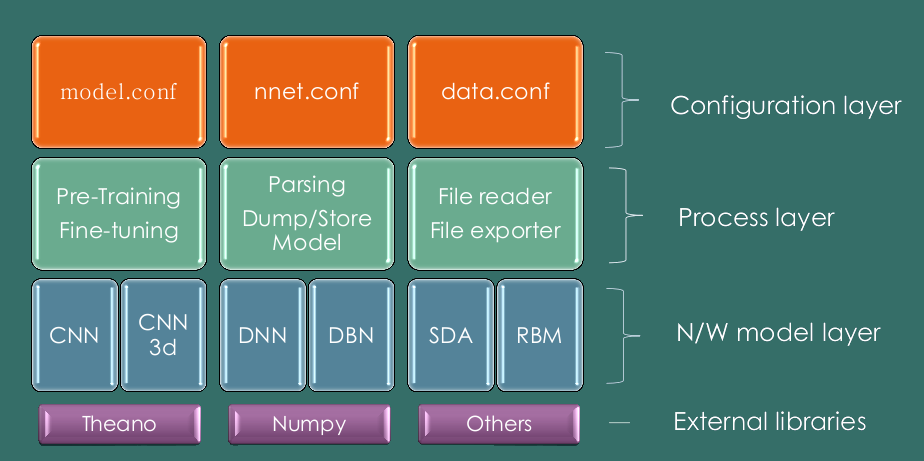
\includegraphics[width=\textwidth]{./img/architecture.png}
			\caption{Python DNN toolkit\footnotemark architecture.}
		\end{figure}
	\end{column}
	\begin{column}{0.4\textwidth}
		\begin{varblock}[\textwidth]{Features}
			\begin{itemize}							
				\item Allows easy configuration of the model.
				\item Run seamlessly on CPU and GPU machines.
				\item Supports CNN, CNN-3D, DNN, DBN, SDA, RBM.			
			\end{itemize}
		\end{varblock}
	\end{column}
\end{columns}
\footnotetext[5]{\tiny{\textbf{github : } (\url{https://github.com/IITM-DONLAB/python-dnn})}}
\end{frame}
\begin{frame}{\textbf{Background Subtraction}}

\begin{columns}
	\begin{column}{0.48\textwidth}
		\begin{varblock}[\textwidth]{Objective}
			To identify pixels that contribute to motion.
		\end{varblock}
		\begin{varblock}[\textwidth]{Approaches\cite{piccardi}}
			\begin{itemize}							
				\item Frame Differencing~~\href{run:videos/bgsub/fd.avi}{{\color{red}[video]}}
				\item Mixture of Gaussian~\href{run:videos/bgsub/mog.avi}{{\color{red}[video]}}
				\item \textit{\color{blue}Eigen Subtraction}~~~\href{run:videos/bgsub/es.avi}{{\color{red}[video]}}		
			\end{itemize}
		\end{varblock}
	\end{column}
	\begin{column}{0.49\textwidth}
		\begin{figure}
			\begin{framed}
			\centering
				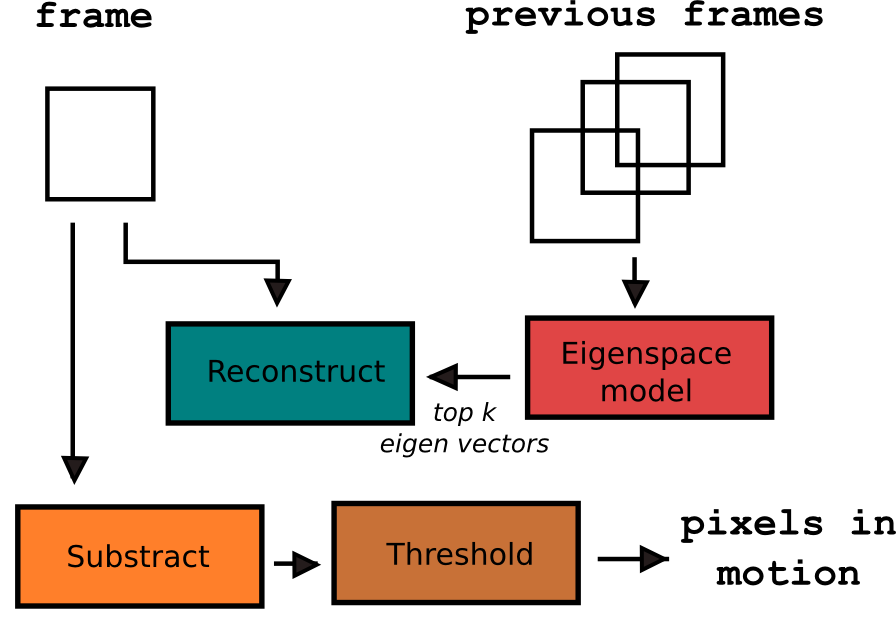
\includegraphics[width=0.75\textwidth]{./img/eigensub.png}
			\end{framed}
			\caption{Flow diagram of Eigen Subtraction.}
		\end{figure}
	\end{column}
\end{columns}
\end{frame}